\documentclass[10pt,a4paper]{report}
\usepackage[utf8]{inputenc}
\usepackage{amsmath}
\usepackage{amsfonts}
\usepackage{amssymb}
\usepackage{graphicx}
\usepackage{float}
\author{Group 5:\\Manoj Velmurugan,AE14B013,\\Mohamed Khalid, AE13B013,\\Radhakrishnan B, AE14B024,\\Mohamed Ajmal, AE14B043,\\G.D.Sunil,AE13B049 }
\title{Spacecraft dynamics project to design a zero momentum biased satellite.}
\begin{document}
\maketitle
\tableofcontents
\part{Problem Statement}
Design a preliminary attitude control system for a satellite. The satellite can have any of the following stabilisation methods given below.
\begin{enumerate}
\item Gravity gradient stabilisation
\item Spin/dual spin stabilisation with passive/active magnetic torque for damping. 
\item Momentum biased stabilisers with earth sensors measuring roll and pitch as primary sensors with gyroscopes and schemes for momentum dumping using thrusters.
\item 0 momentum biased spacecraft with star sensor for roll, pitch and yaw euler parameters with gyroscopes along with momentum dumping mechanism of wheels.\\
\\
\end{enumerate}

\emph{\textbf{Steps involved:}}
\begin{enumerate}
\item Select a suitable kinematic system for spacecraft.
\item Using Euler's equation derive dynamical equations of motion and include gravity gradient torque.
\item Study stability dynamics of the system of both pitch motion and roll-
yaw motion and figure out what kind of motion is possible. Also describe why active control system is required.
\item Design a control system accordingly to control spacecraft with PID strategies.
\item Figure out a control strategy to momentum dump with selected wheel based control.
\item Select proportional control gain accounting for maximum allowable steady state 
of 0.005 deg about all axes (for zero-momentum biased system).

\end{enumerate}

\textbf{Problem Assigned:}\\
Oceansat-1 is a 3-axis stabilized earth pointing satellite with a 4-wheel configuration which is traditional. That is the wheel configuration is with a wheel about each principal axis and the 4th wheel is mounted with 54.7 deg with respect to all three wheels. Nominally the principal axis wheels are rotated with 1000 rpm and the redundant wheel is rotated with -1732 rpm so that zero-momentum is achieved.
\begin{figure}[H]
\centering
\includegraphics[scale=0.5]{untitled.png}
\caption{Configuration of wheels}
\end{figure}
The momentum dumping is achieved by using 60 Am$ ^{2} $ torque rods about all the three axes. Actual MI properties of the s/c after deployment are,
\begin{equation}
J_{c}=\begin{bmatrix}
1800 & -50 & -15 \\
-50 & 1600 & 25 \\
-15 & 25 & 1200 \\
\end{bmatrix} Kg m^{2}
\end{equation}
Where the mass is given to be 1600 Kg, and [x,y,z] correspond to yaw, roll and pitch axes respectively.\\ \\
Initially assume that the cross product of inertias is negligible and design
the control system. Then when you actually apply the control, use the
actual inertia matrix and compare and comment how the performance
varies.
\\ \\
Use momentum dumping by torque rods about 2 axes and design PID control for $ T_{x}= T_{z}=2*10^{-3}Nm $ and $ T_{y}=10^{-4}Nm $ with $ \omega_{0}= 1.0741*10^{-3} rad/s $.
Also compare strategy and time responses for tetrahedron and Pyramid configurations.
\\\begin{figure}[H]
\centering
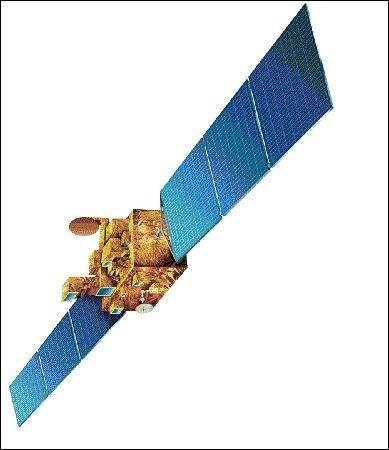
\includegraphics[scale=0.5]{image_gallery.png}
\caption{Ocean Sat}
\end{figure}
\part{Kinematics of spacecraft}
The kinematics for the spacecraft is modelled using Euler angles since the spacecraft is expected to operate within small ranges of Euler angles and it is easier to model the desired orientation using the Euler angles convention.
\\ \\
The Dynamical Equations of motion for the spacecraft are given as follows.\\
\begin{equation}
I\dot{\omega_{b}}+\left(\omega_{b}-C_{b0}\begin{bmatrix}
0\\0\\\omega_{0}
\end{bmatrix}\right)\times(I\left(\omega_{b}-C_{b0}\begin{bmatrix}
0\\0\\\omega_{0}
\end{bmatrix}\right)=T_{disturbance}+T_{magnetic}-T_{RW}
\end{equation}

Where T represents Torque and $ T_{magnetic} $ represents torque by magnetic torquers due to momentum dumping and $ T_{RW} $ represents torque due to reaction wheels.
\\
\\
For reaction wheels, the net torque due to the wheels come out as,
\begin{equation}
T_{RW}=I_{w}\begin{bmatrix}
\dot{\omega_{1}}-\frac{\omega_{4}}{\sqrt{3}}\\
\dot{\omega_{2}}-\frac{\omega_{4}}{\sqrt{3}}\\
\dot{\omega_{3}}-\frac{\omega_{4}}{\sqrt{3}}
\end{bmatrix}
+I_{w}\begin{bmatrix}
\omega_{3}\omega_{by}-\omega_{2}\omega_{bz}\\
\omega_{1}\omega_{bz}-\omega_{3}\omega_{bx}\\
\omega_{2}\omega_{bx}-\omega_{1}\omega_{by}
\end{bmatrix}
\end{equation}
Where,
\end{document}